\documentclass[]{article}
\usepackage[table, dvipsnames]{xcolor}% http://ctan.org/pkg/xcolor
\usepackage{fullpage} % Package to use full page
\usepackage{parskip} % Package to tweak paragraph skipping
\usepackage{tikz} % Package for drawing
\usepackage{amsmath}
\usepackage{hyperref}




\title{Introduction to Arduino and the LCD Display  --  Hello, World!}
\author{Dr. Matthew Riehl}


\begin{document}

\newcommand{\tc}{\textcolor}

\maketitle
%{today}

\section{Introduction}

For the next several weeks, we will be building circuits to investigate the properties of resistors, capacitors,  and other electronic components.  In order to do this, we  first build a simple device that will be used to help us gather our data in later labs.

\emph{Note that this is NOT a programming class (no previous programming experience is needed); the code is provided and can be used without editing (although you are encouraged to play with the code to extend the functionality of the device\dots). Neither is this a circuits class; we will not be exploring the details of how the Arduino and other components work.  Of course, we hope that this taste of programming and bread-boarding inspire you to take additional courses in computer science or electronics\dots}

This week, we will set up the Arduino to send a  message to the LCD display.  You will wire the LCD to the Arduino with the breadboard and jumper wires and use your computer to compile the code that will control the display. This code will be sent to the Arduino which will execute the code until it is turned off or until the code is replaced with a different set of instructions.  Once the code has been stored on the Arduino, it can be disconnected from the computer and powered by any appropriate source.

In later labs, we will modify the circuit to gather data which will be displayed on the LCD screen.  This has the benefit of allowing you to see what is going on inside the circuit to some extent.  The downside is that any changes you make to your circuit or experiment will have to be coded into the program and loaded onto the Arduino.  

\section{Materials}

\begin{itemize}
	\item Computer with Arduino IDE installed (\href{https://www.arduino.cc/en/software}{arduino.cc/en/software}\footnote{for this exercise, Arduino IDE 1.8.15 was used})
	\item Arduino Uno board and power cable
	\item Half-size breadboard
	\item LCD display module
	\item 220 $\Omega$ resistor ($\Omega$ is Ohm)
	\item 10 k$\Omega$ potentiometer
	\item Jumper wires
\end{itemize}

\section{Wiring the LCD to the Arduino}

We will build circuits by copying diagrams given in the laboratory handout.  In some cases, the functions of pins will be described, but mostly we will leave the details to the engineers and programmers who designed the boards and accessories.  Pin-out diagrams of the Arduino Uno (Figure \ref{ArduinoPinOut}) and the LCD board (Figure \ref{fig2}) are shown. 

	\begin{figure}
	\begin{tikzpicture}[scale=0.85]
		\node[anchor=south west,inner sep=0] (image) at (0,0) {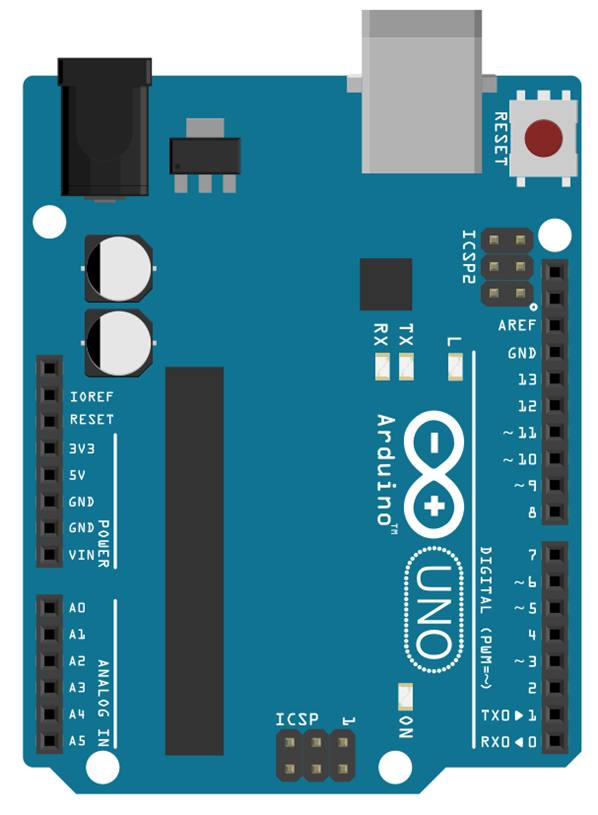
\includegraphics[width=0.438\textwidth]{pics/arduino}};
		%%%% Node placement %%%%
		\node [anchor=east] (ref) at (0,5.97) {\small I/O Reference voltage};
		\node [anchor=east] (reset) at (0,5.593) {\small Reset};
		\node [anchor=east] (lowv) at (0,5.217) {\small 3.3V Output};
		\node [anchor=east] (highv) at (0,4.84) {\small 5V Output};
		\node [anchor=east] (ground1) at (0,4.46) {\small Ground};
		\node [anchor=east] (ground2) at (0,4.086) {\small Ground};
		\node [anchor=east] (inputv) at (0,3.71) {\small Input voltage};
		%
		\node [anchor=east] (ap0) at (0,2.95) {\small Analog pin 0};
		\node [anchor=east] (ap1) at (0,2.573) {\small Analog pin 1};
		\node [anchor=east] (ap2) at (0,2.196) {\small Analog pin 2};
		\node [anchor=east] (ap3) at (0,1.82) {\small Analog pin 3};
		\node [anchor=east] (sda) at (0,1.443) {\small Analog 4 (I2C) SDA};
		\node [anchor=east] (scl) at (0,1.066) {\small Analog 5 (I2C) SCL};
		%
		% Right side pins
		\node [anchor=west] (aref) at (9,6.97) {\small Analog Reference voltage};
		\node [anchor=west] (ground3) at (9,6.59) {\small Ground};
		\node [anchor=west] (dp13) at (9,6.21) {\small Digital pin 13};
		\node [anchor=west] (dp12) at (9,5.83) {\small Digital pin 12};
		\node [anchor=west] (dp11) at (9,5.45) {\small Digital pin 11, PWM};
		\node [anchor=west] (dp10) at (9,5.07) {\small Digital pin 10, PWM};
		\node [anchor=west] (dp9) at (9,4.69) {\small Digital pin 9, PWM};
		\node [anchor=west] (dp8) at (9,4.31) {\small Digital pin 8};
		%
		\node [anchor=west] (dp7) at (9,3.72) {\small Digital pin 7};
		\node [anchor=west] (dp6) at (9,3.341) {\small Digital pin 6, PWM};
		\node [anchor=west] (dp5) at (9,2.962) {\small Digital pin 5, PWM};
		\node [anchor=west] (dp4) at (9,2.582) {\small Digital pin 4};
		\node [anchor=west] (dp3) at (9,2.203) {\small Digital pin 3, PWM};
		\node [anchor=west] (dp2) at (9,1.824) {\small Digital pin 3, PWM};
		\node [anchor=west] (tx) at (9,1.445) {\small Communication with computer};
		\node [anchor=west] (rx) at (9,1.066) {\small Communication with computer};
		
		%%%% Arrow placement %%%%
		\draw[-latex, red, ultra thick] (ref) -- (0.75,5.97);
		\draw[-latex, red, ultra thick] (reset) -- (0.75,5.593);
		\draw[-latex, red, ultra thick] (lowv) -- (0.75,5.217);
		\draw[-latex, red, ultra thick] (highv) -- (0.75,4.84);
		\draw[-latex, red, ultra thick] (ground1) -- (0.75,4.46);
		\draw[-latex, red, ultra thick] (ground2) -- (0.75,4.086);
		\draw[-latex, red, ultra thick] (inputv) -- (0.75,3.71);
		%
		\draw[-latex, red, ultra thick] (ap0) -- (0.75,2.95);
		\draw[-latex, red, ultra thick] (ap1) -- (0.75,2.573);
		\draw[-latex, red, ultra thick] (ap2) -- (0.75,2.196);
		\draw[-latex, red, ultra thick] (ap3) -- (0.75,1.82);
		\draw[-latex, red, ultra thick] (sda) -- (0.75,1.443);
		\draw[-latex, red, ultra thick] (scl) -- (0.75,1.066);
		% 
		\draw[-latex, red, ultra thick] (aref) -- (8,6.97);
		\draw[-latex, red, ultra thick] (ground3) -- (8,6.59);
		\draw[-latex, red, ultra thick] (dp13) -- (8,6.21);
		\draw[-latex, red, ultra thick] (dp12) -- (8,5.83);
		\draw[-latex, red, ultra thick] (dp11) -- (8,5.45);
		\draw[-latex, red, ultra thick] (dp10) -- (8,5.07);
		\draw[-latex, red, ultra thick] (dp9) -- (8,4.69);
		\draw[-latex, red, ultra thick] (dp8) -- (8,4.31);
		%
		\draw[-latex, red, ultra thick] (dp7) -- (8,3.74);
		\draw[-latex, red, ultra thick] (dp6) -- (8,3.341);
		\draw[-latex, red, ultra thick] (dp5) -- (8,2.962);
		\draw[-latex, red, ultra thick] (dp4) -- (8,2.582);
		\draw[-latex, red, ultra thick] (dp3) -- (8,2.203);
		\draw[-latex, red, ultra thick] (dp2) -- (8,1.824);
		\draw[-latex, red, ultra thick] (tx) -- (8,1.445);
		\draw[-latex, red, ultra thick] (rx) -- (8,1.066);
	\end{tikzpicture}
	\caption{Pin-out Diagram for the Arduino Uno.  PWM is Pulse Width Modulation}
	\label{ArduinoPinOut}
\end{figure}

Some pins will not be used for our projects.

\begin{figure}
	\centering
	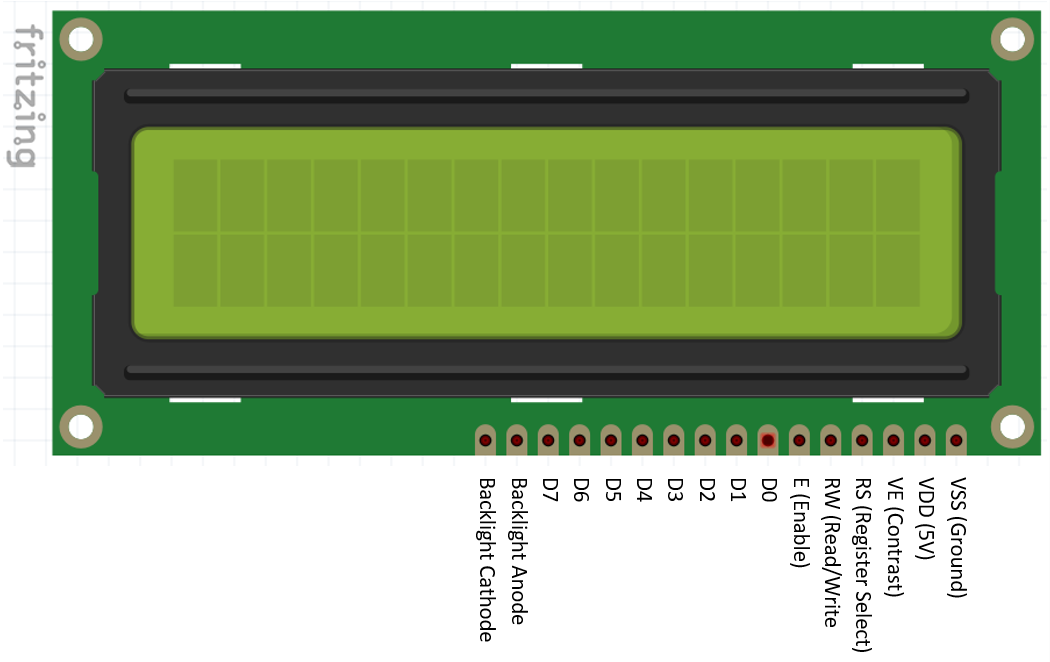
\includegraphics[width=10cm]{pics/lcd pinout.png}
	\caption{Pin-out Diagram for the LCD}
	\label{fig2}
\end{figure}

\begin{figure}
	\centering
	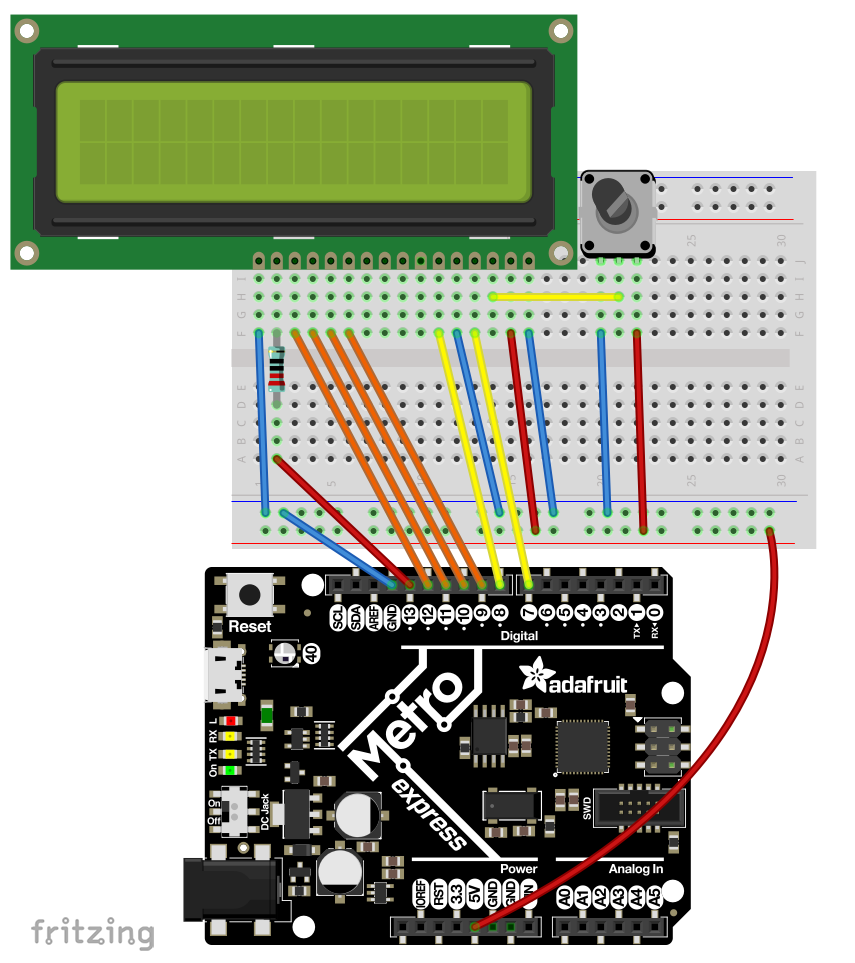
\includegraphics[width=10cm]{pics/lcd wiring.png}
	\caption{Hello World Wiring Diagram}
	\label{HelloWorld}
\end{figure}

The wiring diagram is shown in Figure \ref{HelloWorld}.  It is useful to use the color of wire suggested in the diagram, because it will be  easier to troubleshoot if the board does not work.  It is suggested that you wire the breadboard first (black, red, and blue wires) and then connect the Arduino with final wires.  If you have some experience with the Arduino, you might notice that the LCD wiring in this project is a bit different than what you have seen online.  The wiring shown here is more clear and the code has been changed to reflect the changes.

You will need to find a 220$\Omega$ resistor.  The resistance of each resistor is coded on the body of the resistor by means of a series of colored bands.  Most resistors have either 4 bands or 5 bands.  See figure \ref{Colorchart} for a description of the resistors and the colors used and figure \ref{resistor} for an example of how to read the bands.


\section{Code for the Arduino}

The code for Arduino is written in the computer language "C++", which is one of the most common languages in use.  The code that will be used today is given below.  Note that the text that occurs between 
/* 
and 
*/
are comments, not part of the actual code.  Also, any line that begins with // is a comment. If you delete all of the comments, the code is quite small.

This code is in the file Arduino\_Basic\_Hello\_World.ino.  The file will open in the Arduino IDE.  The file Arduino\_Hello\_World.ino demonstrates a number of commands available for the LCD.  
\bigskip


\begin{verbatim}
/*
LiquidCrystal Library - Hello World

This code is included with the files for Arduino Lab Hello World by 
Matthew Riehl and is in the public domain.  I have only modified the
code to better support the laboratory exercise.

Demonstrates the use a 16x2 LCD display.  The LiquidCrystal
library works with all LCD displays that are compatible with the
Hitachi HD44780 driver. There are many of them out there, and you
can usually tell them by the 16-pin interface.

This sketch prints "Hello World!" to the LCD
and shows the number of seconds since reset.

Note that the pin assignments are NOT the same as found on many Arduino 
pages.  They have been moved around to make the wiring more intuitive 
and easier to troubleshoot.

The circuit:
* LCD RS pin to digital pin 7
* LCD Enable pin to digital pin 8
* LCD D4 pin to digital pin 9
* LCD D5 pin to digital pin 10
* LCD D6 pin to digital pin 11
* LCD D7 pin to digital pin 12
* LCD Backlight (pin 15 on LCD) to pin 13 on Arduino (might need to add a 220 ohm series resistor)
* LCD R/W pin to ground
* LCD VSS pin to ground
* LCD VCC pin to 5V
* 10K potentiostat:
* ends to +5V and ground
* wiper to LCD VO pin (pin 3)

Library originally added 18 Apr 2008
by David A. Mellis
library modified 5 Jul 2009
by Limor Fried (http://www.ladyada.net)
example added 9 Jul 2009
by Tom Igoe
modified 22 Nov 2010
by Tom Igoe
modified 7 Nov 2016
by Arturo Guadalupi

This example code is in the public domain.

http://www.arduino.cc/en/Tutorial/LiquidCrystalHelloWorld

*/

// include the library code:
#include <LiquidCrystal.h>

// initialize the library by associating any needed LCD interface pin
// with the arduino pin number it is connected to
const int rs = 7, en = 8, d4 = 9, d5 = 10, d6 = 11, d7 = 12;
LiquidCrystal lcd(rs, en, d4, d5, d6, d7);
#define backlightPin 13         // This allows the user to turn the back light on and off.

void setup() {
	// set up the LCD's number of columns and rows:
	lcd.begin(16, 2);
	// Print a message to the LCD.
	pinMode(backlightPin, OUTPUT);
	digitalWrite(backlightPin, HIGH);
	lcd.print("Hello, World!");       // Change this to something cool!
	
}
void loop() {
	// set the cursor to column 0, line 1
	// (note: line 1 is the second row, since counting begins with 0):
	lcd.setCursor(0, 1);
	// print the number of seconds since reset:
	lcd.print(millis() / 1000);
}
\end{verbatim}





\section{Hello World Program in the Arduino IDE}

Open the Arduino IDE, identified by the logo shown in Figure \ref{arduino}.  Open the \textbf{ File$>$Examples$>$01.Basics$>$Blink} and wait for the code to appear in a new window.  Read through the comments which explain what the program does and which parts of the code control the output.


\begin{figure}[h]
	\centering
	
\includegraphics[width=6cm]{pics/arduino-ide.png}
	\caption{Arduino Logo}
	\label{arduino}
\end{figure}

Connect the Arduino to the computer with the cable.  Under the Tools menu in the IDE, find the Board Manager and select your board (Arduino Uno) and then find the Port menu and ensure that the IDE is connected to the Arduino Uno port.  Under the Sketch menu, choose Upload and wait until the routine is over.  If no errors are encountered, a small LED on the Arduino will be blinking on and off in one second intervals.  Now change the timing on the blinking and upload your new program to see the new blink pattern.  This sketch does not use the LCD, which will remain off.

Open the file 
Arduino\_Basic\_Hello\_World by double clicking icon.  It will open in a new Arduino IDE window.  It should be identical to the code above. Upload this sketch as it is and ensure that it is working.  The LCD should display a message on the first line and be counting seconds on the second line.  It may be necessary to change the setting on the potentiometer in order to see the screen with proper contrast.  

Now, the file Arduino\_Hello\_World.ino can be opened and uploaded to the Arduino.  Take some time to read the code and try to modify it to see what it can do.  More details on how the commands work can be found online (see the links in the comment section of the program)-- this project is not intended to teach the details of programming.  


	\begin{figure}
	\begin{center}
		\renewcommand*{\arraystretch}{1.2}
		\begin{tabular}{cccccc}
			\hline
			Color & \(1^{\text{st}}\) Band & \(2^{\text{nd}}\) Band & \(3^{\text{rd}}\) Band & Multiplier & Tolerance \\ \hline
			\rowcolor{black} \tc{white}{\textbf{Black}} & \tc{white}{0} & \tc{white}{0} & \tc{white}{0} & \tc{white}{\(1 \Omega\)} &  \\
			\rowcolor{brown} \textbf{Brown} & 1 & 1 & 1 & \(10 \Omega\) & \(\pm 1\%\) \\
			\rowcolor{red} \textbf{Red} & 2 & 2 & 2 & \(100 \Omega\) & \(\pm 2\%\) \\
			\rowcolor{orange} \textbf{Orange} & 3 & 3 & 3 & \(1 \text{k}\Omega\) &  \\
			\rowcolor{yellow} \textbf{Yellow} & 4 & 4 & 4 &\(10 \text{k}\Omega\)  &  \\
			\rowcolor{green} \textbf{Green} & 5 & 5 & 5 & \(100 \text{k}\Omega\) & \(\pm 0.5\%\) \\
			\rowcolor{blue} \tc{white}{\textbf{Blue}} & \tc{white}{6} & \tc{white}{6} & \tc{white}{6} & \tc{white}{\(1 \text{M}\Omega\)} & \tc{white}{\(\pm 0.25\%\)} \\
			\rowcolor{violet} \tc{white}{\textbf{Violet}} & \tc{white}{7} & \tc{white}{7} & \tc{white}{7} & \tc{white}{\(10 \text{M}\Omega\)} & \tc{white}{\(\pm 0.10\%\)} \\
			\rowcolor{black!50} \tc{white}{\textbf{Grey}} & \tc{white}{8} & \tc{white}{8} & \tc{white}{8} & \tc{white}{\(100 \text{M}\Omega\)} & \tc{white}{\(\pm 0.05\%\)} \\
			\rowcolor{white} \textbf{White} & 9 & 9 & 9 & \(1 \text{G}\Omega\) &  \\
			\rowcolor{Dandelion} \textbf{Gold} &  &  &  & \(0.1 \Omega\) & \(\pm 5\%\) \\
			\rowcolor{black!25} \textbf{Silver} &  &  &  & \(0.01 \Omega\) & \(\pm 10\%\) \\ \hline
		\end{tabular}
		\caption{Color banding codes for resistors}
		\label{Colorchart}
	\end{center}
	\end{figure}

	\begin{figure}
		\centering
		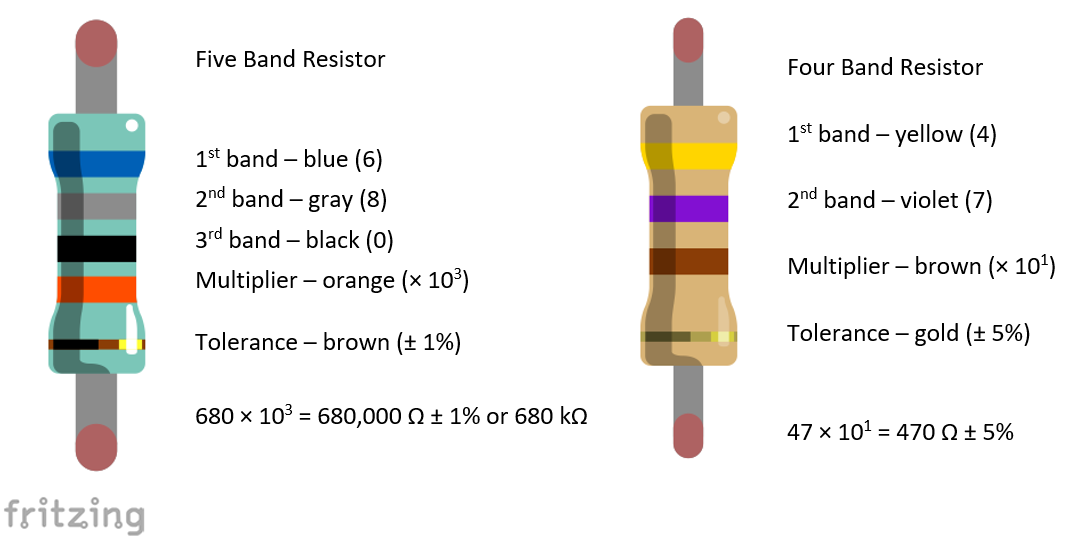
\includegraphics[width=12cm]{pics/resistor.png}
		\caption{Examples of a 5-band and 4-band resistor}
		\label{resistor}
	\end{figure}

\end{document}
